\documentclass[a4paper, 12pt]{article}
\usepackage[margin=2cm]{geometry} 
\usepackage{amsmath,amsfonts}
\usepackage{amssymb,amsthm}
\usepackage{tikz,tkz-euclide}
\usepackage[cm]{fullpage}
\usepackage{fancyvrb}

\usetikzlibrary{calc,patterns,angles,quotes}
\usetkzobj{all}

\title{Senior Test 3}
\author{Stellenbosch Camp 2018}
\date{Time: $2 \frac{1}{2}$ hours}

\begin{document} \maketitle

\begin{enumerate}
% 2017/2018 British MO Round 2 Q1
\item[1.] Let $ABC$ be a triangle, and let the midpoint of $AC$ be $M$. The circle tangent to $BC$ at $B$ and passing through $M$ meets the line $AB$ again at $P$. Prove that $AB \times BP = 2 BM^2$.
\vspace{7pt}

% The Aether
\item[2.]
Show that for all positive real numbers $x$ and $y$,
\[ \frac{x^2}{x+2y} +\frac{y^2}{2x+y} \geq \frac{x+y}{3}. \]
\vspace{5pt}

% (Iberoamerican Mathematical Olympiad shortlist 2009)
\item[3.]
Consider an $8 \times 8$ grid of squares. On each square is a lightbulb which is initially switched off. A move consists of choosing a square and either the vertical or horizontal direction, and toggling the lightbulb on that square and it's immediate neighbours in the chosen direction. For clarity this means that usually 3 bulbs are flipped unless the square is on an edge in which case 2 bulbs may be flipped. After some amount of moves a single bulb is switched on (the other 63 are off). Determine which of the 64 bulbs can possibly be on. 
\vspace{7pt}

% 2017/2018 British MO Round 2
\item[4.]
Determine whether or not there is a positive integer $m$ such that
\[ (m+1)^3 +(m+2)^3 +\dotsb +(2m)^3 \]
is a square.

\vspace{7pt}

% Hong Kong Team Selection Test 2, 21 October 2017
\item[5.]  In triangle $ABC$ with incentre $I$, let $M_A, M_B$ and $M_C$ be the midpoints of $BC$, $CA$, and $AB$ respectively, and $H_A$, $H_B$, and $H_C$ be the feet of altitudes from $A, B$ and $C$ to the respective sides. Denote by $l_b$ the line being tangent to the circumcircle of triangle $ABC$ and passing through $B$, and denote by $l_b'$ the reflection of $l_b$ in $BI$. Let $P_B$ be the intersection of $M_A M_C$ and $l_b$, and let $Q_B$ be the intersection of $H_A H_C$ and $l_b'$. Define $l_c, l_c', P_C$ and $Q_C$ analogously. If $R$ is the intersection of $P_B Q_B$ and $P_C Q_C$, prove that $RB = RC$.

\end{enumerate}

\vfill

%  Should be box and whiskers diagram here
\begin{figure}[h]
	\centering
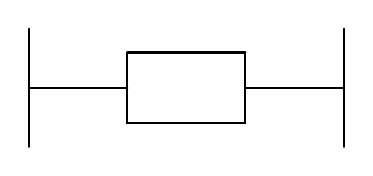
\begin{tikzpicture}[scale=0.25]
\tkzDefPoints{-8/3/o1, -8/-3/o2, 8/3/o3, 8/-3/o4, -3/1.8/o5, -3/-1.8/o6, 3/1.8/o7, 3/-1.8/o8,-3/0/w1, 3/0/w2, -8/0/w3, 8/0/w4}
\tkzDrawSegments[thick](o1,o2 o3,o4 o5,o6 o7,o8 o5,o7 o6,o8 w1,w3 w2,w4)

\end{tikzpicture}
\caption{This is \textbf{not} real math.}
\end{figure}

\vspace{12mm}

\end{document}
